% generated by report/gen_tables.py from build/scene_export.json -- do not edit
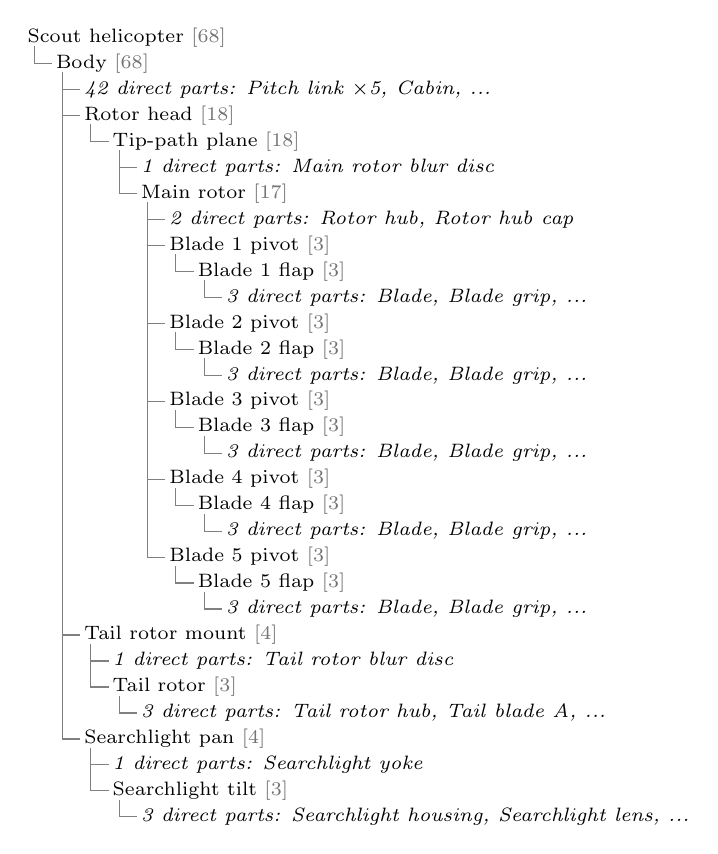
\begin{tikzpicture}[x=0.36cm,y=-0.33cm,font=\scriptsize]
\node[anchor=west,inner sep=0pt] (n0) at (0,0) {Scout helicopter \textcolor{black!55}{[68]}};
\node[anchor=west,inner sep=0pt] (n1) at (1,1) {Body \textcolor{black!55}{[68]}};
\draw[black!50,thin] (0.25,0.35) |- (0.88,1);
\node[anchor=west,inner sep=0pt] (n2) at (2,2) {\textit{42 direct parts: Pitch link $\times$5, Cabin, ...}};
\draw[black!50,thin] (1.25,1.35) |- (1.88,2);
\node[anchor=west,inner sep=0pt] (n3) at (2,3) {Rotor head \textcolor{black!55}{[18]}};
\draw[black!50,thin] (1.25,1.35) |- (1.88,3);
\node[anchor=west,inner sep=0pt] (n4) at (3,4) {Tip-path plane \textcolor{black!55}{[18]}};
\draw[black!50,thin] (2.25,3.35) |- (2.88,4);
\node[anchor=west,inner sep=0pt] (n5) at (4,5) {\textit{1 direct parts: Main rotor blur disc}};
\draw[black!50,thin] (3.25,4.35) |- (3.88,5);
\node[anchor=west,inner sep=0pt] (n6) at (4,6) {Main rotor \textcolor{black!55}{[17]}};
\draw[black!50,thin] (3.25,4.35) |- (3.88,6);
\node[anchor=west,inner sep=0pt] (n7) at (5,7) {\textit{2 direct parts: Rotor hub, Rotor hub cap}};
\draw[black!50,thin] (4.25,6.35) |- (4.88,7);
\node[anchor=west,inner sep=0pt] (n8) at (5,8) {Blade 1 pivot \textcolor{black!55}{[3]}};
\draw[black!50,thin] (4.25,6.35) |- (4.88,8);
\node[anchor=west,inner sep=0pt] (n9) at (6,9) {Blade 1 flap \textcolor{black!55}{[3]}};
\draw[black!50,thin] (5.25,8.35) |- (5.88,9);
\node[anchor=west,inner sep=0pt] (n10) at (7,10) {\textit{3 direct parts: Blade, Blade grip, ...}};
\draw[black!50,thin] (6.25,9.35) |- (6.88,10);
\node[anchor=west,inner sep=0pt] (n11) at (5,11) {Blade 2 pivot \textcolor{black!55}{[3]}};
\draw[black!50,thin] (4.25,6.35) |- (4.88,11);
\node[anchor=west,inner sep=0pt] (n12) at (6,12) {Blade 2 flap \textcolor{black!55}{[3]}};
\draw[black!50,thin] (5.25,11.35) |- (5.88,12);
\node[anchor=west,inner sep=0pt] (n13) at (7,13) {\textit{3 direct parts: Blade, Blade grip, ...}};
\draw[black!50,thin] (6.25,12.35) |- (6.88,13);
\node[anchor=west,inner sep=0pt] (n14) at (5,14) {Blade 3 pivot \textcolor{black!55}{[3]}};
\draw[black!50,thin] (4.25,6.35) |- (4.88,14);
\node[anchor=west,inner sep=0pt] (n15) at (6,15) {Blade 3 flap \textcolor{black!55}{[3]}};
\draw[black!50,thin] (5.25,14.35) |- (5.88,15);
\node[anchor=west,inner sep=0pt] (n16) at (7,16) {\textit{3 direct parts: Blade, Blade grip, ...}};
\draw[black!50,thin] (6.25,15.35) |- (6.88,16);
\node[anchor=west,inner sep=0pt] (n17) at (5,17) {Blade 4 pivot \textcolor{black!55}{[3]}};
\draw[black!50,thin] (4.25,6.35) |- (4.88,17);
\node[anchor=west,inner sep=0pt] (n18) at (6,18) {Blade 4 flap \textcolor{black!55}{[3]}};
\draw[black!50,thin] (5.25,17.35) |- (5.88,18);
\node[anchor=west,inner sep=0pt] (n19) at (7,19) {\textit{3 direct parts: Blade, Blade grip, ...}};
\draw[black!50,thin] (6.25,18.35) |- (6.88,19);
\node[anchor=west,inner sep=0pt] (n20) at (5,20) {Blade 5 pivot \textcolor{black!55}{[3]}};
\draw[black!50,thin] (4.25,6.35) |- (4.88,20);
\node[anchor=west,inner sep=0pt] (n21) at (6,21) {Blade 5 flap \textcolor{black!55}{[3]}};
\draw[black!50,thin] (5.25,20.35) |- (5.88,21);
\node[anchor=west,inner sep=0pt] (n22) at (7,22) {\textit{3 direct parts: Blade, Blade grip, ...}};
\draw[black!50,thin] (6.25,21.35) |- (6.88,22);
\node[anchor=west,inner sep=0pt] (n23) at (2,23) {Tail rotor mount \textcolor{black!55}{[4]}};
\draw[black!50,thin] (1.25,1.35) |- (1.88,23);
\node[anchor=west,inner sep=0pt] (n24) at (3,24) {\textit{1 direct parts: Tail rotor blur disc}};
\draw[black!50,thin] (2.25,23.35) |- (2.88,24);
\node[anchor=west,inner sep=0pt] (n25) at (3,25) {Tail rotor \textcolor{black!55}{[3]}};
\draw[black!50,thin] (2.25,23.35) |- (2.88,25);
\node[anchor=west,inner sep=0pt] (n26) at (4,26) {\textit{3 direct parts: Tail rotor hub, Tail blade A, ...}};
\draw[black!50,thin] (3.25,25.35) |- (3.88,26);
\node[anchor=west,inner sep=0pt] (n27) at (2,27) {Searchlight pan \textcolor{black!55}{[4]}};
\draw[black!50,thin] (1.25,1.35) |- (1.88,27);
\node[anchor=west,inner sep=0pt] (n28) at (3,28) {\textit{1 direct parts: Searchlight yoke}};
\draw[black!50,thin] (2.25,27.35) |- (2.88,28);
\node[anchor=west,inner sep=0pt] (n29) at (3,29) {Searchlight tilt \textcolor{black!55}{[3]}};
\draw[black!50,thin] (2.25,27.35) |- (2.88,29);
\node[anchor=west,inner sep=0pt] (n30) at (4,30) {\textit{3 direct parts: Searchlight housing, Searchlight lens, ...}};
\draw[black!50,thin] (3.25,29.35) |- (3.88,30);
\end{tikzpicture}
